%!TEX root = ../../dissertation.tex
%%%%%%%%%%%%%%%%%%%%%%%%%%%%%%%%%%%%%%%%%%%%%%%%%%%%%%%%%%%%%%%%%%%%%%%%%%%%%%%
\section{Load Model Queuing Simulation} 
\label{c4:simulation}

As discussed, the solvability of a non-stationary Erlang loss system is very limited. To better tackle this, a simulative approach kann be taken. Depending on the level of detail, different types of simulations are available.

Here, a queuing simulation is used to ascertain the blocking probability and tunnel serving slot utilization from the model using the fitted distributions from the trace.


%%
\subsection{Queuing Simulation Implementation}

The queuing simulation is implemented on the basis of a \gls{DES}. Instead of reproducing continuous time, this simulation is a series of discrete events. Time is advanced only at these events. 

A queuing model can be easily represented in a \gls{DES}.  Each tunnel request arrival is a modeled as a discrete event. When such an event occurs, three processes are executed. The first process draws a random number from a \gls{PRNG} mapped to \gls{IAT} exponential distribution to schedule the next arrival event. Secondly, the serving units are checked for any free units. If one is found, it will now be occuppied. Else, this arrival will be marked as rejected and the third action skipped. This third process now determines the length of the tunnel using another \gls{PRNG} adjusted to the serving time distribution to schedule the event in which the tunnel exits the system.

This model was implemented on the basis of version 3.0 of the \textit{SimPy}~\cite{simpy} package, which is a Python \gls{DES} framework that provides the basic event and scheduling infrastructure. On top of this a base \gls{GGSN} class was constructed, managing the arrival of tunnel events and the scheduling of the service ending events. Specific clases for the traditional (i.e. monolithic) and virtualized (called ``multiserver'' in the code) nodes respectively exist. The implementation is also publicly available\footnote{\url{https://github.com/fmetzger/ggsn-simulation/}} as a reference. 


To be in line with the measurement data the simulation time is set to be \SI{7}{\day} for all simulation scenarios. The initial \SI{60}{\minute} are considered to be the transient phase and are dedacted from the results. Ten replications of each scenario were performed. All error bars given in this section show the \SI{5}{\percent} and \SI{95}{\percent} quantiles of all replications.

The first round of simulations were conducted solely to find appropriate simulation parametersas a baseline for all further studies. Thereafter, further rounds using the monolithic \gls{GGSN} were conducted. With these, the scaling and load of the node in relation to the tunnel arrivals can be investigated.

Based on these results, the virtualization and scaling out effects  through the second, virtualized \gls{GGSN} model are examined. In a final extended experiment the the startup and shutdown duration of virtual instances are taken into account to increase the realism.


%%
\subsection{Traditional GGSN}
\label{c4:sec:eval_traditional_ggsn}

With the help of the interarrival times and duration of tunnels we study the traditional \gls{GGSN} model previously introduced. Whilst our measurements provided us with information on the frequency of new tunnels and the duration they remain active, we have no reliable information on the number of active tunnels the \gls{GGSN} can support. Thus, in a first step, we dimension the \gls{GGSN} in such a way that a suitable blocking probability $p_B$ can be achieved.

\begin{figure}[htb]
  \centering
    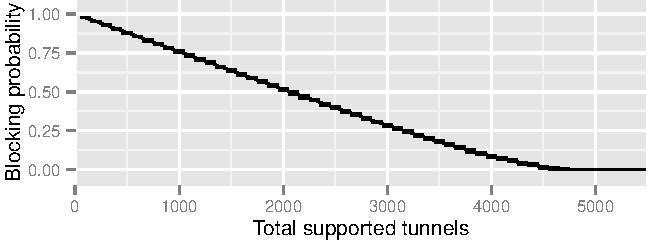
\includegraphics[width=1.0\textwidth]{images/traditional-blocking.pdf}
  \caption{Impact of the number of supported parallel tunnels on the blocking probability for the traditional \gls{GGSN} model. For each scenario the mean of all simulated replications as well as \SI{5}{\percent} and \SI{95}{\percent} quantiles as error bars are shown.}
  \label{c4:fig:traditional_blocking}
\end{figure}

In Figure~\ref{c4:fig:traditional_blocking} the maximum number of tunnels $n$, that can be active simultaneously, is gradually increased to study the impact on the blocking probability $p_B$. We observe, that as the number of supported parallel tunnels increases, the blocking probability decreases. For the normalized interarrival no blocking is occurring if we allow for more than $5000$ parallel tunnels. Thus, we consider the range of $4000$ to $5000$ parallel tunnels to be of special interest for the remainder of the study.


%%
\subsection{Virtual \texorpdfstring{\acrshort{GGSN}}{GGSN}}
\label{c4:sec:eval_ideal_virtual_ggsn}

\todo{hypervisor start/stop ruleset descripiton}
For example, one could always hold one instance in reserve for upcoming requests and provision as soon as the reserve gets used. Similar rules should apply in the shutdown of servers and should form a hysteresis together with the boot condition. 
For example it would be possible to keep at least one server in reserve but never more than two.

In order to study the feasibility of the virtual \gls{GGSN} approach discussed in Sec.~\ref{c4:sec:virtual_ggsn}, we compare the performance indicators of the virtual \gls{GGSN} with that of a traditional \gls{GGSN}. To this end, the virtual \gls{GGSN} is simulated in varying configurations.
The number of servers and supported tunnels per server is chosen in such a way that the results can be compared with those obtained from our study of the traditional \gls{GGSN}. Due to simulation time constraints, only a representative subset of scenarios is simulated.

In the virtual \gls{GGSN} model, servers are activated and deactivated on demand, while in the traditional \gls{GGSN} model, the single server is always on. For this investigation a conservative start up and shut down time of \SI{300}{\second} is chosen. Generally, deactivating server instances reduces energy consumption and frees up inactive servers for other use. For this reason, the number of active servers is a relevant performance metric in the virtual \gls{GGSN} model.


\begin{table}[htb]
	\caption{Manipulation check for the experimental factors based on one-way ANOVA.}
	\centering
	\label{c4:tab:manipulation2color}
	\begin{tabu}{X[l]X[r]X[r]X[r]XX}%{lrrrcc}
	\toprule
	& \multicolumn{1}{c}{$\mathbf{F(2,1275)}$} & \multicolumn{1}{c}{$\mathbf{\eta^2_p}$} & \multicolumn{1}{c}{$\mathbf{p}$} & \textbf{Cohen's} & \textbf{Cohen's}\\ 
	&  & & & $\mathbf{f^2}$ & $\mathbf{\hat{\omega}^2}$ \\ 
	\midrule
	\emph{blocking probability}  & & & & &\\ 
	maxTunnels &  $15601.534$ & $\color{red} 0.99$ & $<0.001$ & $\color{red} 26.739$ & $0.964$\\ 
	maxInstances &  $10218.173$ & $\color{red} 0.986$ & $<0.001$ & $\color{red} 1.068$ & $0.516$\\ 
	startstopDuration &  $0.868$ & $\color{black} 0.003$ & $0.482$ & $\color{black} 0.000$ & $0.000$\\ 
	\midrule
	\emph{mean number of tunnels}  & & & & &\\ 
	maxTunnels &  $20448.347$ & $\color{red} 0.994$ & $<0.001$ & $\color{red} 27.712$ & $0.965$\\ 
	maxInstances &  $13348.251$ & $\color{red} 0.989$ & $<0.001$ & $\color{red} 1.064$ & $0.515$\\ 
	startstopDuration &  $2.872$ & $\color{black} 0.009$ & $0.022$ & $\color{black} 0.000$ & $0.000$\\ 
	\bottomrule
	\end{tabu}
\end{table}

In order to analyze the influence of the different model parameters on the performance metrics, we perform a one-way ANOVA analysis with the results in Table~\ref{c4:tab:manipulation2color}. High values for $\eta_p^2$ and Cohen's $f^2$ \cite{stats} indicate that the main influence for both blocking probability and mean number of tunnels is the maximum number of tunnels $n$ and servers $S_{\max}$, i.e. the total number of possible concurrent tunnels in the system.
Therefore, we study these parameters first.

\begin{figure}[htb]
  \centering
  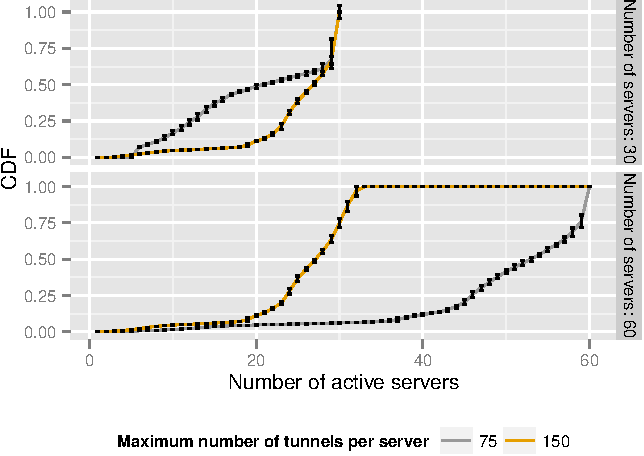
\includegraphics{images/instanceuse-multiserver-real.pdf}
  \caption{Impact of the maximum number of tunnels and number of servers on number of active servers in the virtual \gls{GGSN} model.}
 \label{c4:fig:instance_use_virtual}
\end{figure}

In Figure~\ref{c4:fig:instance_use_virtual} the \gls{CDF} of the number of active servers for four different virtual \gls{GGSN} configurations is displayed. We observe, that increasing the number of supported tunnels per server allows a larger percentage of servers to be shutdown or used for other tasks. This demonstrates the scaling capability of the virtualized model quite well. Note, that both the scenario with $30$ servers and $150$ maximum tunnels per server as well as the scenario with $60$ servers and $75$ maximum tunnels per server share the same maximum amount of tunnels, $4500$, being right at the center of the interesting range of candidates.


\begin{figure}[htb]
  \centering
  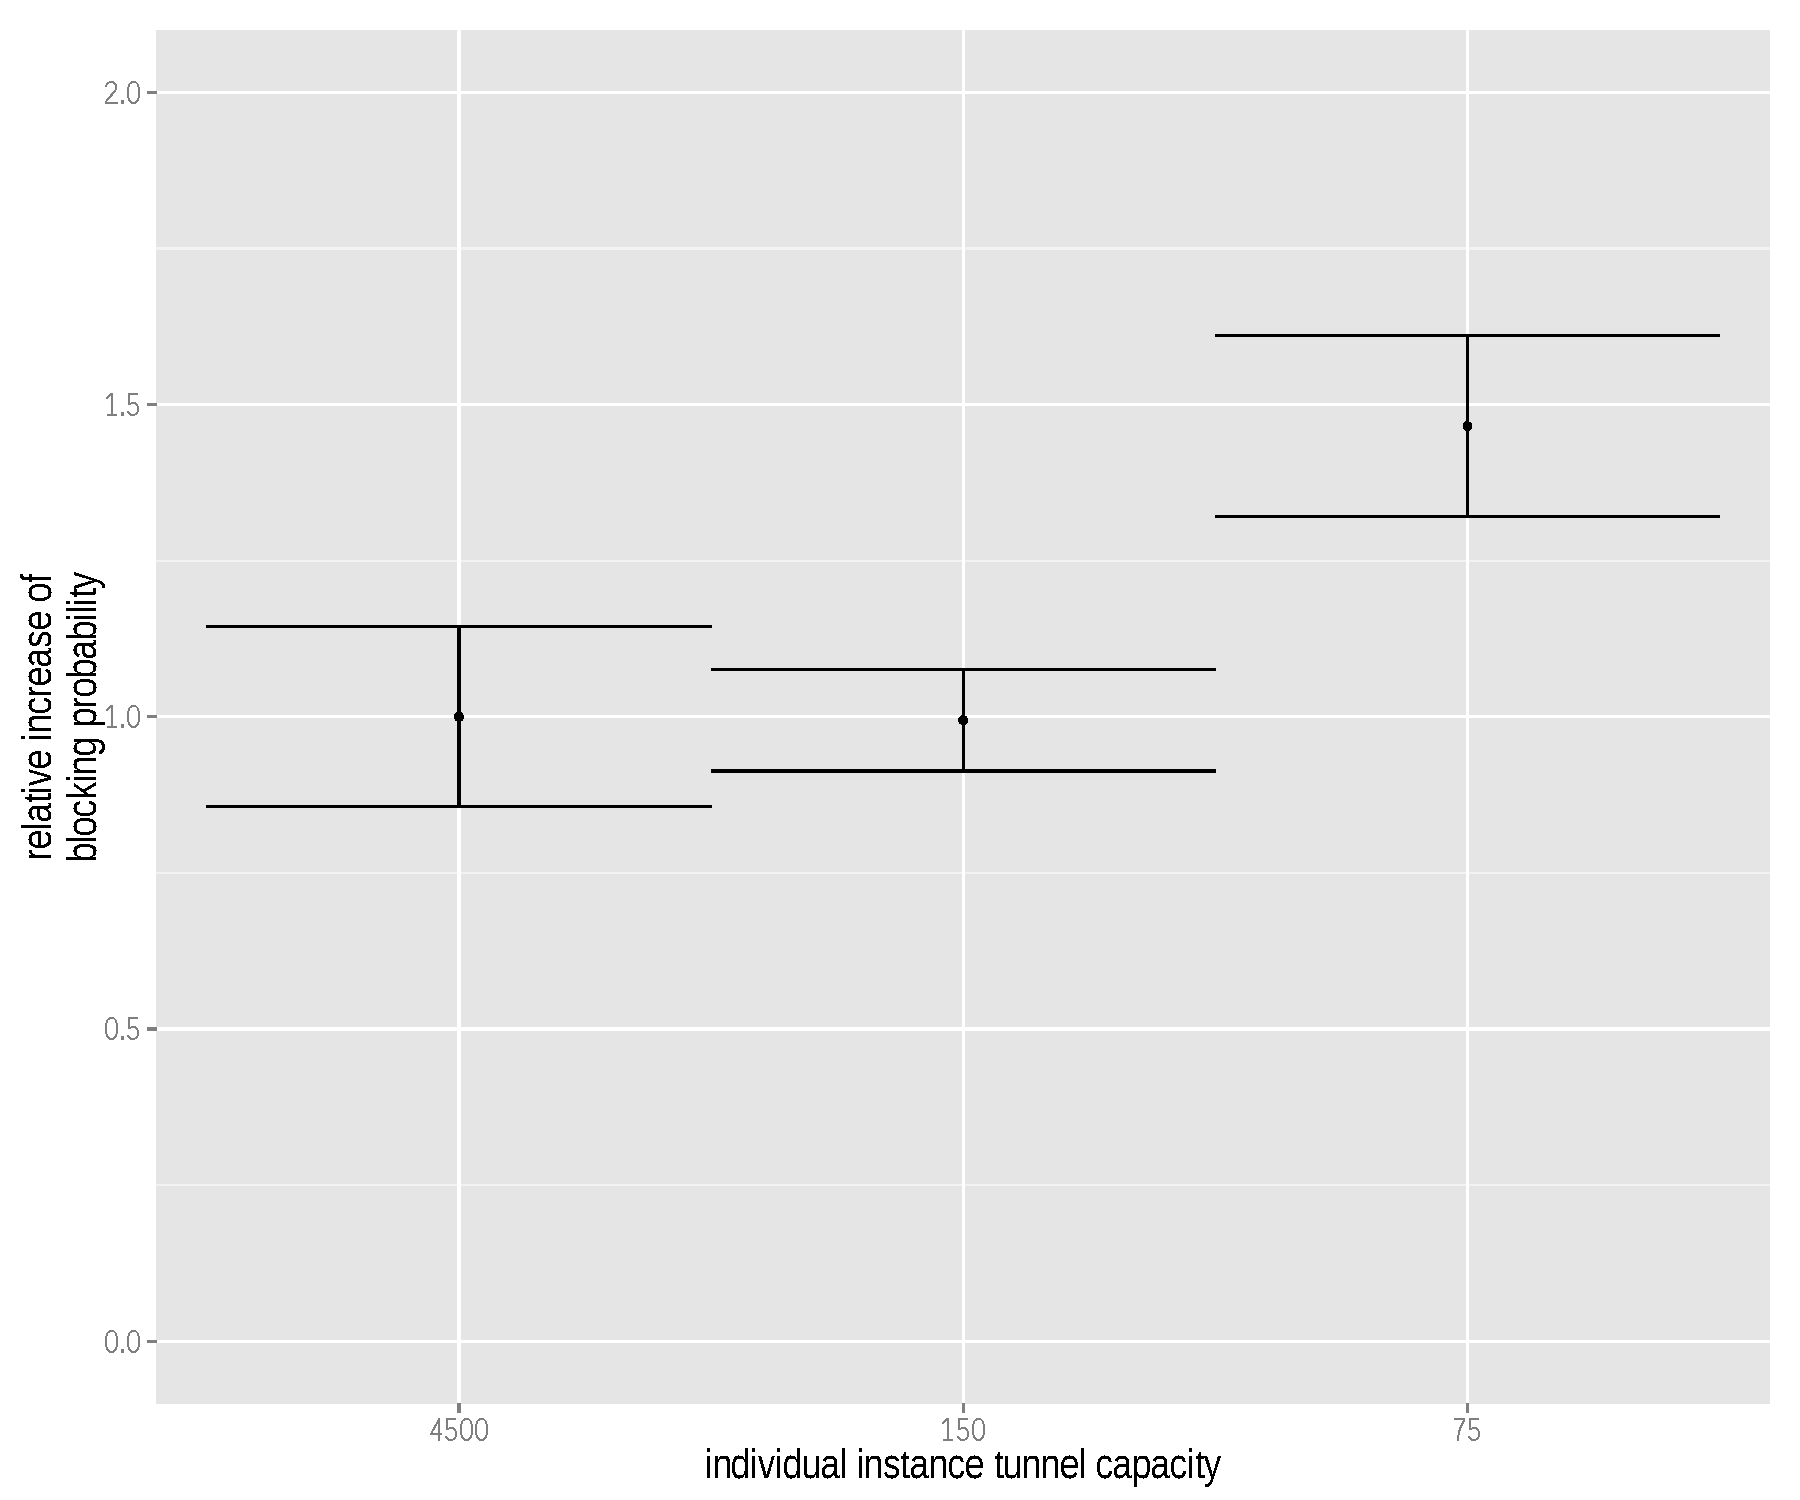
\includegraphics{images/blocking-comparison.pdf}
  \caption{Relative increase of blocking probability on the number of servers compared to the traditional \gls{GGSN}; with the $4500$ maximum tunnels per server being on a single server, $150$ on $30$, and $75$ on $60$ servers.}
 \label{c4:fig:blocking-comparison}
\end{figure}

Next, we take a look at the blocking probability of the virtual \gls{GGSN} system in Figure~\ref{c4:fig:blocking-comparison} and compare it to the results from the traditional \gls{GGSN} model. In Figure~\ref{c4:fig:blocking-comparison} we compare the blocking probability of the traditional \gls{GGSN} system dimensioned for $4500$ concurrent tunnels with the virtual \gls{GGSN}.

We observe that, with the start up and shut down time of $5$ minutes in mind, the blocking probability increases by a factor of $1.48$ if the capacity of each server is set to $75$, i.e. $\frac{1}{60}$ of the original server capacity, while $27$ of all $60$ servers can be turned of or used for other purposes at \SI{50}{\percent} of the time. We conclude, that choosing more powerful servers decreases the blocking probability but reduces the potential to disable servers.

So far we have considered a conservative start up and shut down time of servers of \SI{5}{\minute}, which can potentially occur if current generation physical servers are used.
In the next section we study the impact of reduced start up and shut down times with modern servers with fast storage (e.g. \glspl{SSD}) or virtual servers provisioned in the cloud.


%%
\subsection{Impact of startup and shutdown times}
\label{c4:sec:real_virtual_ggsn}

In this section, we first consider the impact of different boot and shut down times on resource utilization and blocking probabilities. We observe the impact of different start up and shut down times on both resource utilization and blocking probability. Afterwards, the influence of varying server start and stop times on a fixed combination of maximum tunnels and servers in the system is examined.

\begin{figure}[htb]
  \centering
  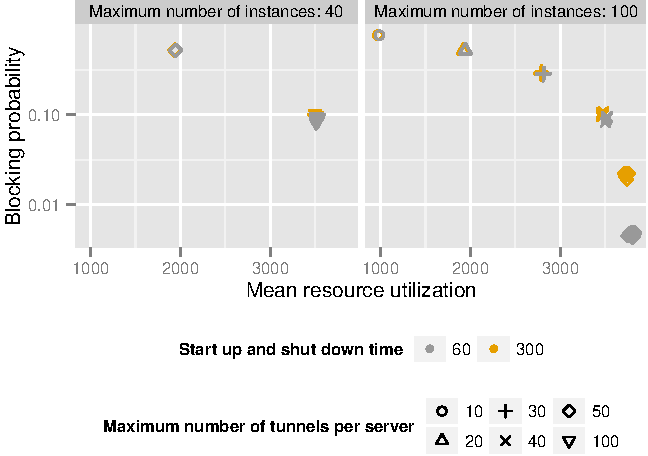
\includegraphics{images/compare-util-block.pdf}
  \caption{Trade-off between blocking probability and mean resource utilization with regard to maximum number of servers, maximum number of tunnels per server, and start up and shut down time.}
 \label{c4:fig:compare_util_block}
\end{figure}

Figure~\ref{c4:fig:compare_util_block} shows scenarios with $40$ and $100$ number of virtual \gls{GGSN} instances and  $1000$ to $5000$ total concurrent tunnels. For each scenario, we study the impact of selecting different maximum numbers of tunnel per server as well as start up and shut down times on blocking probability and mean resource utilization. The first observation is that by increasing the number of servers, i.e. scaling out, the blocking probability can be decreased, while maintaining a relatively low mean resource utilization. In addition to the previous effects, we notice that a higher start up and shut down time causes a slight increase in blocking probability for servers with low tunnel capacity.

\begin{figure}[htb]
  \centering
  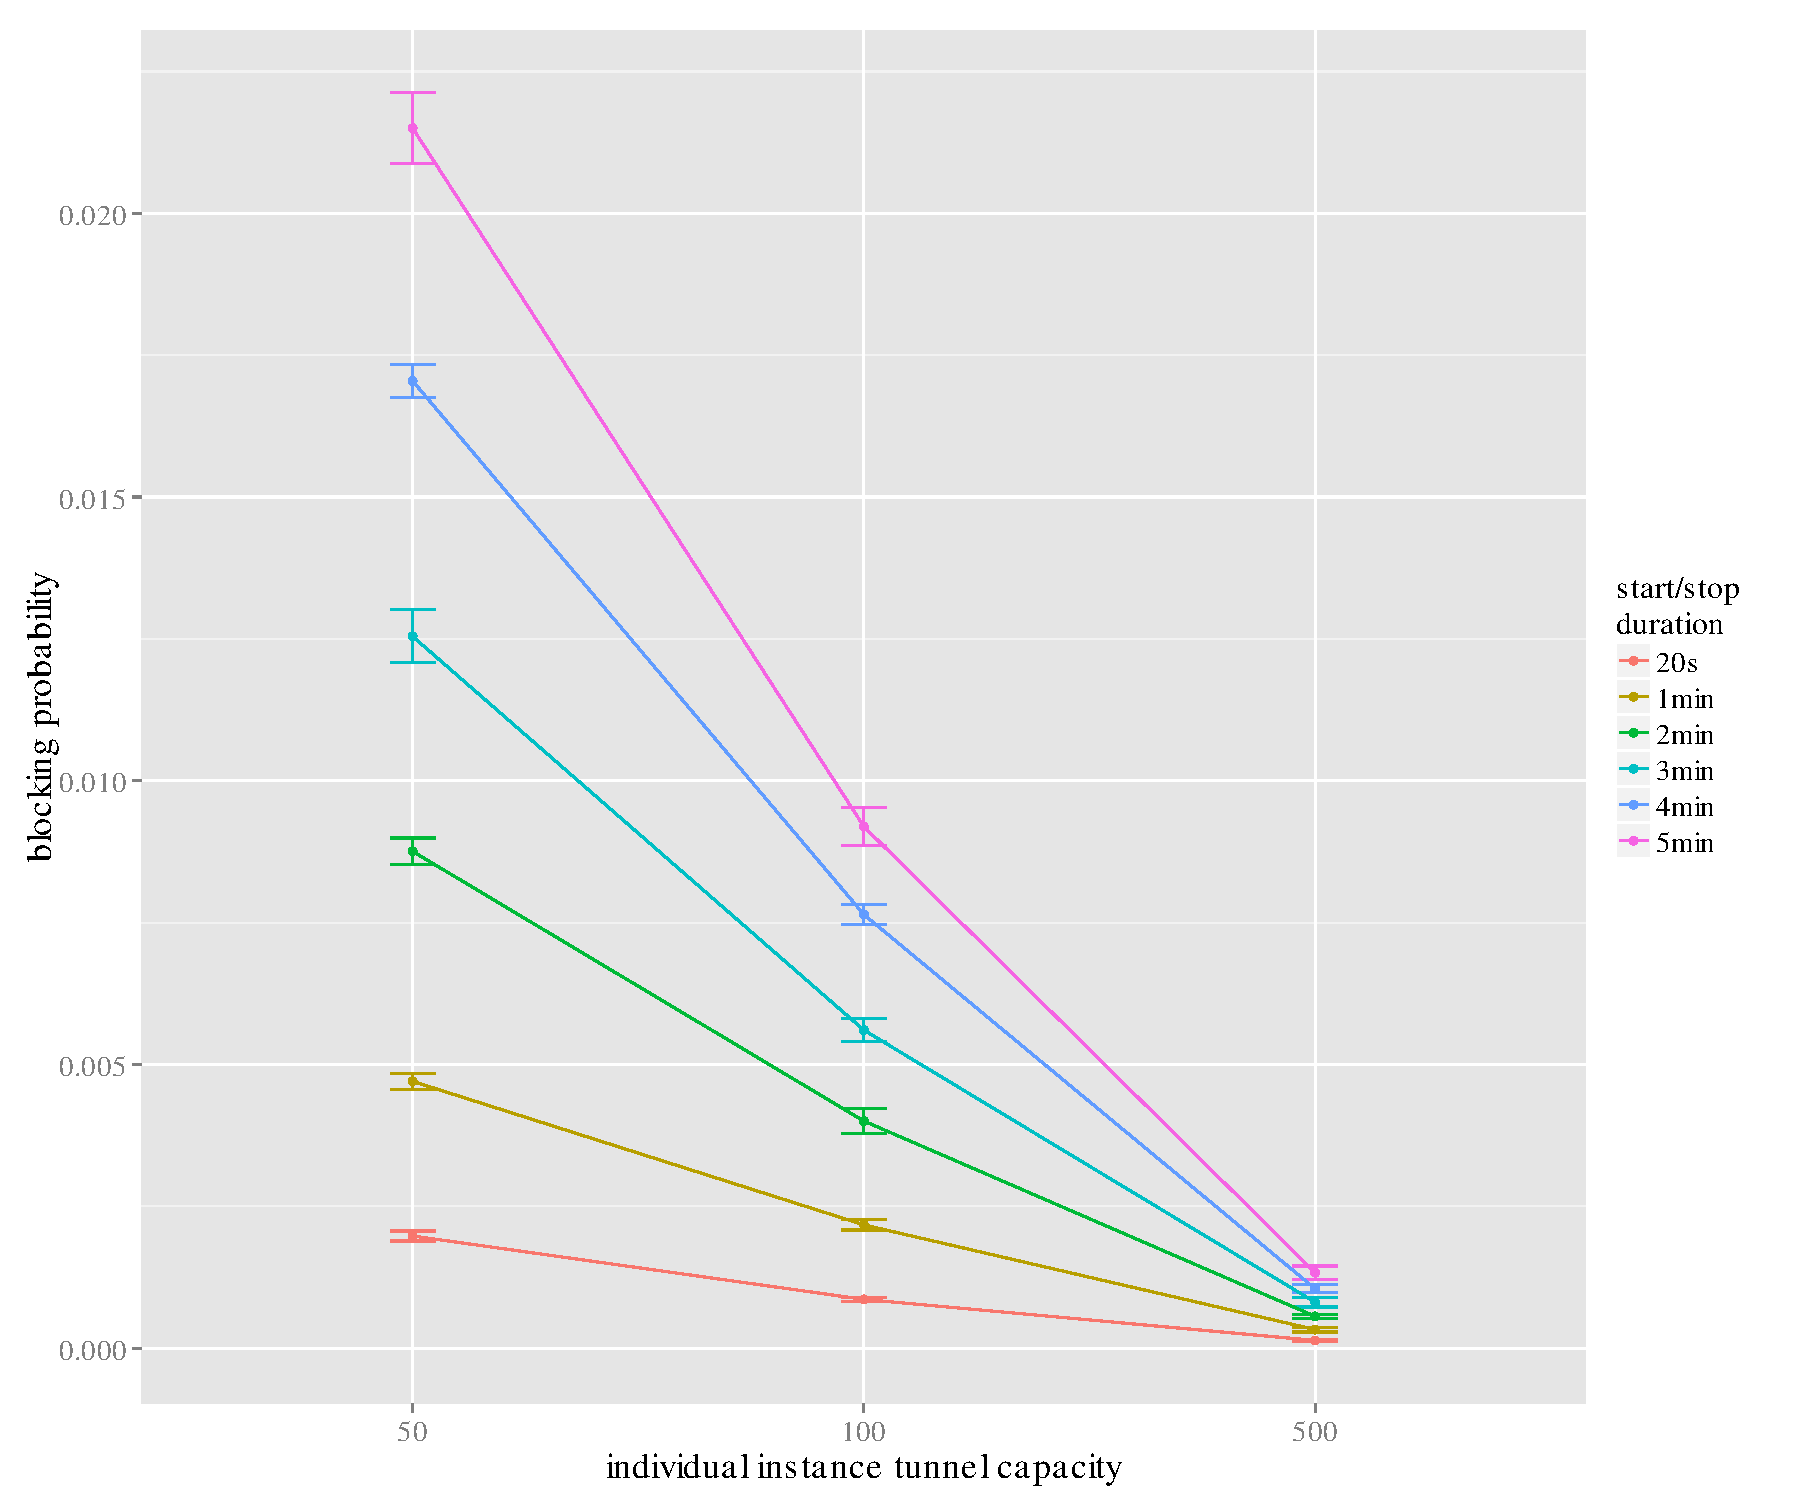
\includegraphics{images/compare-maxinstances-block.pdf}
  \caption{Influence of start up and shut down time on blocking probability with regard to different numbers of servers.}
 \label{c4:fig:compare_maxinstances_block}
\end{figure}

In order to study this behavior in more detail, we focus on a specific scenario in Figure~\ref{c4:fig:compare_maxinstances_block}, where $5000$ total tunnels should be supported by the system. In order to achieve this goal, we consider three types of instances, with the server capacity varying between $50$ and $500$.  In each case we change the start up and shut down time between $1$ and $5$ minutes. It can be easily observed, that lower server capacities combined with higher start up and shut down times increase the blocking probability. This is due to the server start up threshold mechanism, used in the model, not taking the additional capacity gained by activating an additional server into account. If a low capacity server with a long boot time is activated, there is a high probability that the system will quickly expend its capacity again.

Thus, it can be concluded, that if smaller instances are to be used, for example because they are cheaper than large instances, start up and shut down times should be kept minimal, for example by using virtual instances or \glspl{SSD}.




%%%%%%%%%%%%%%%%%%%%%%%%%%%%%%%%%%%%%%%%%%%%%%%%
% additional figures for simulation

\begin{figure}[htb]
  \centering
  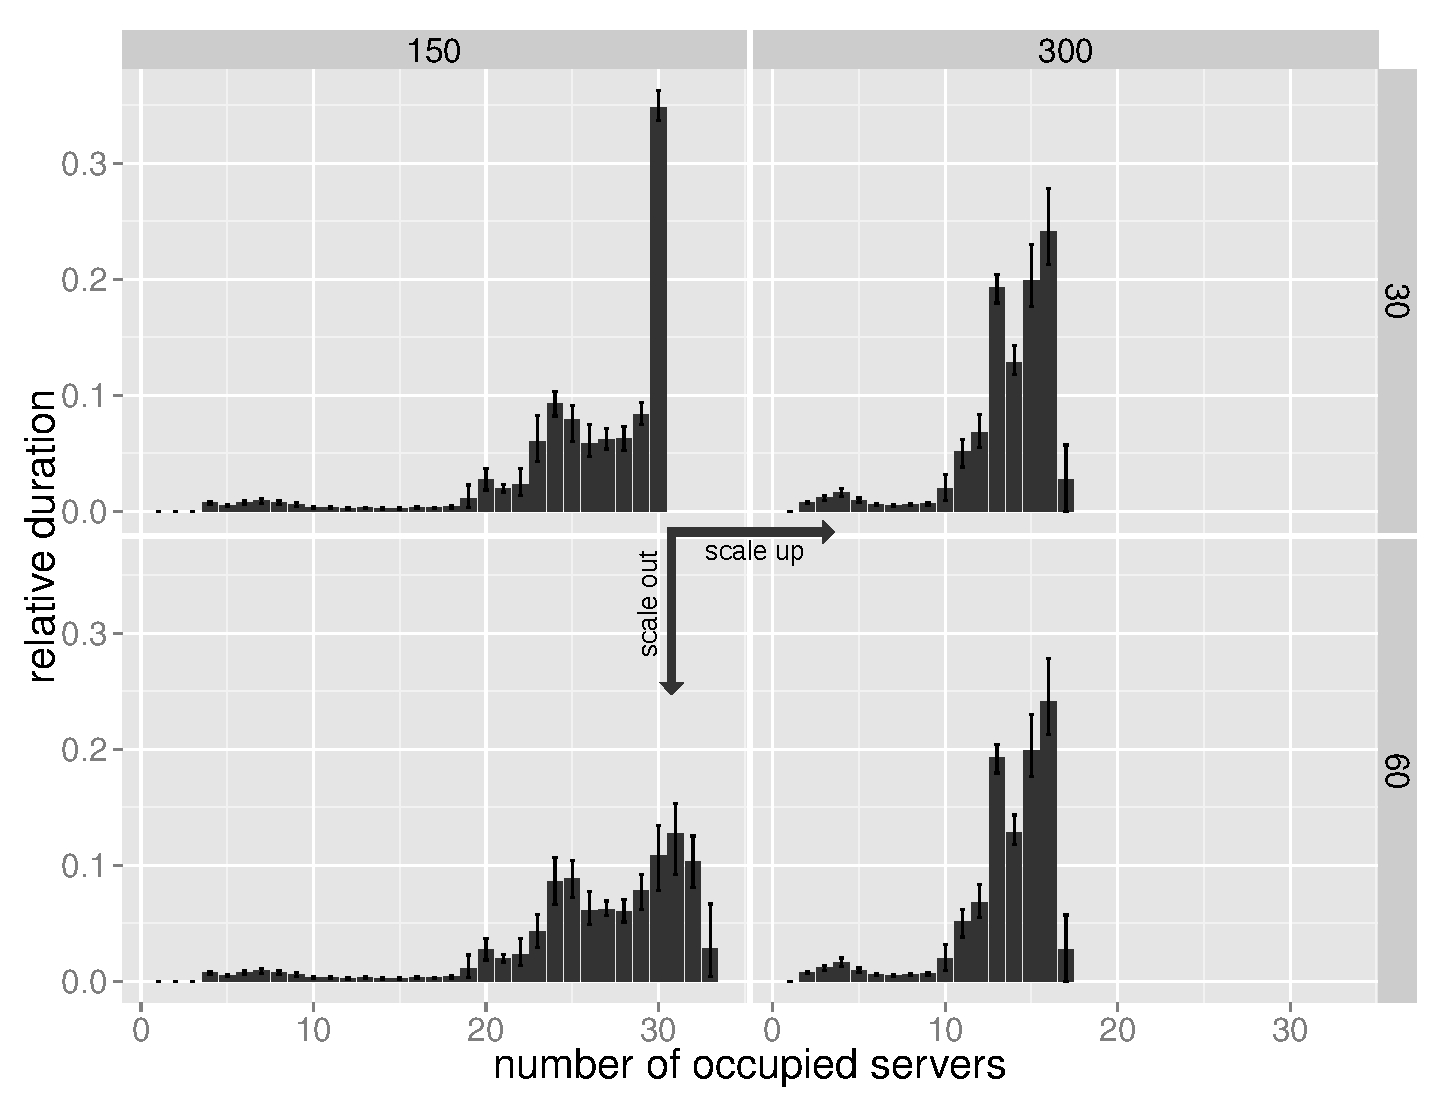
\includegraphics[width=1.0\textwidth]{images/resourceusedistribution-detail-barplot-annotated.pdf}
  \caption{Resource usage from select maximum instances and tunnels combination, displaying the capability to scale.}
 \label{c4:fig:res-usage-barplot}
\end{figure}


\begin{figure}[htb]
  \centering
  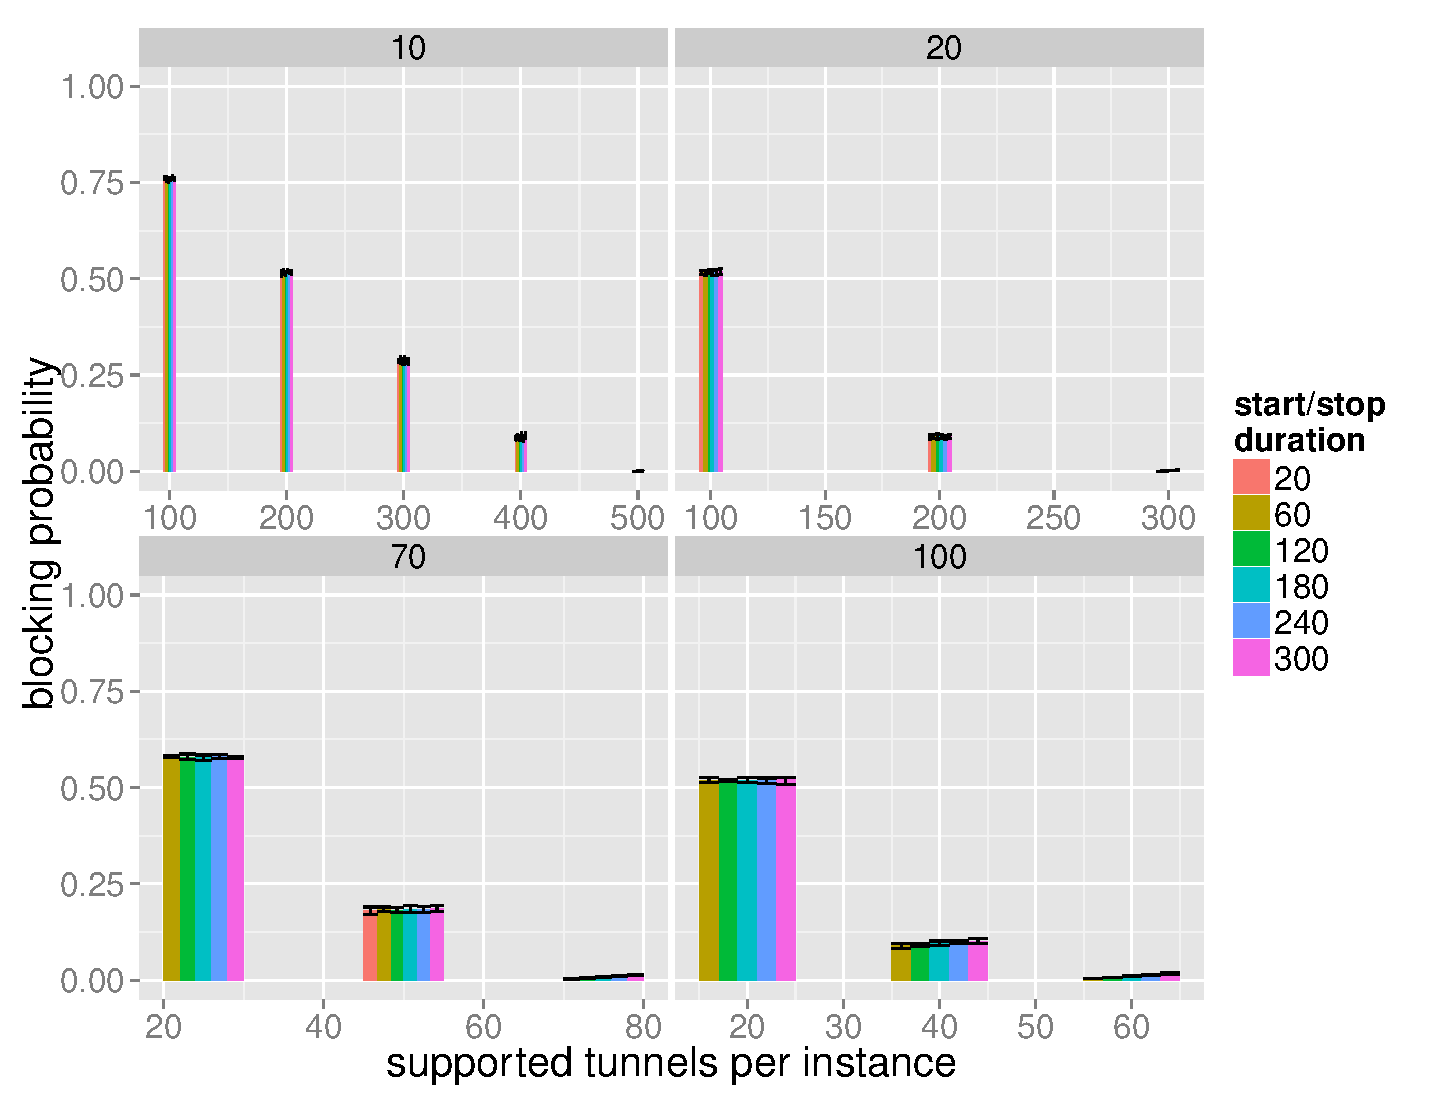
\includegraphics[width=1.0\textwidth]{images/startstopduration-blockingprobability-barchart.pdf}
  \caption{Influence of the boot and shutdown time on the blocking probability.}
 \label{c4:fig:blockprob-startstop-barchart}
\end{figure}

\begin{figure}[htb]
  \centering
  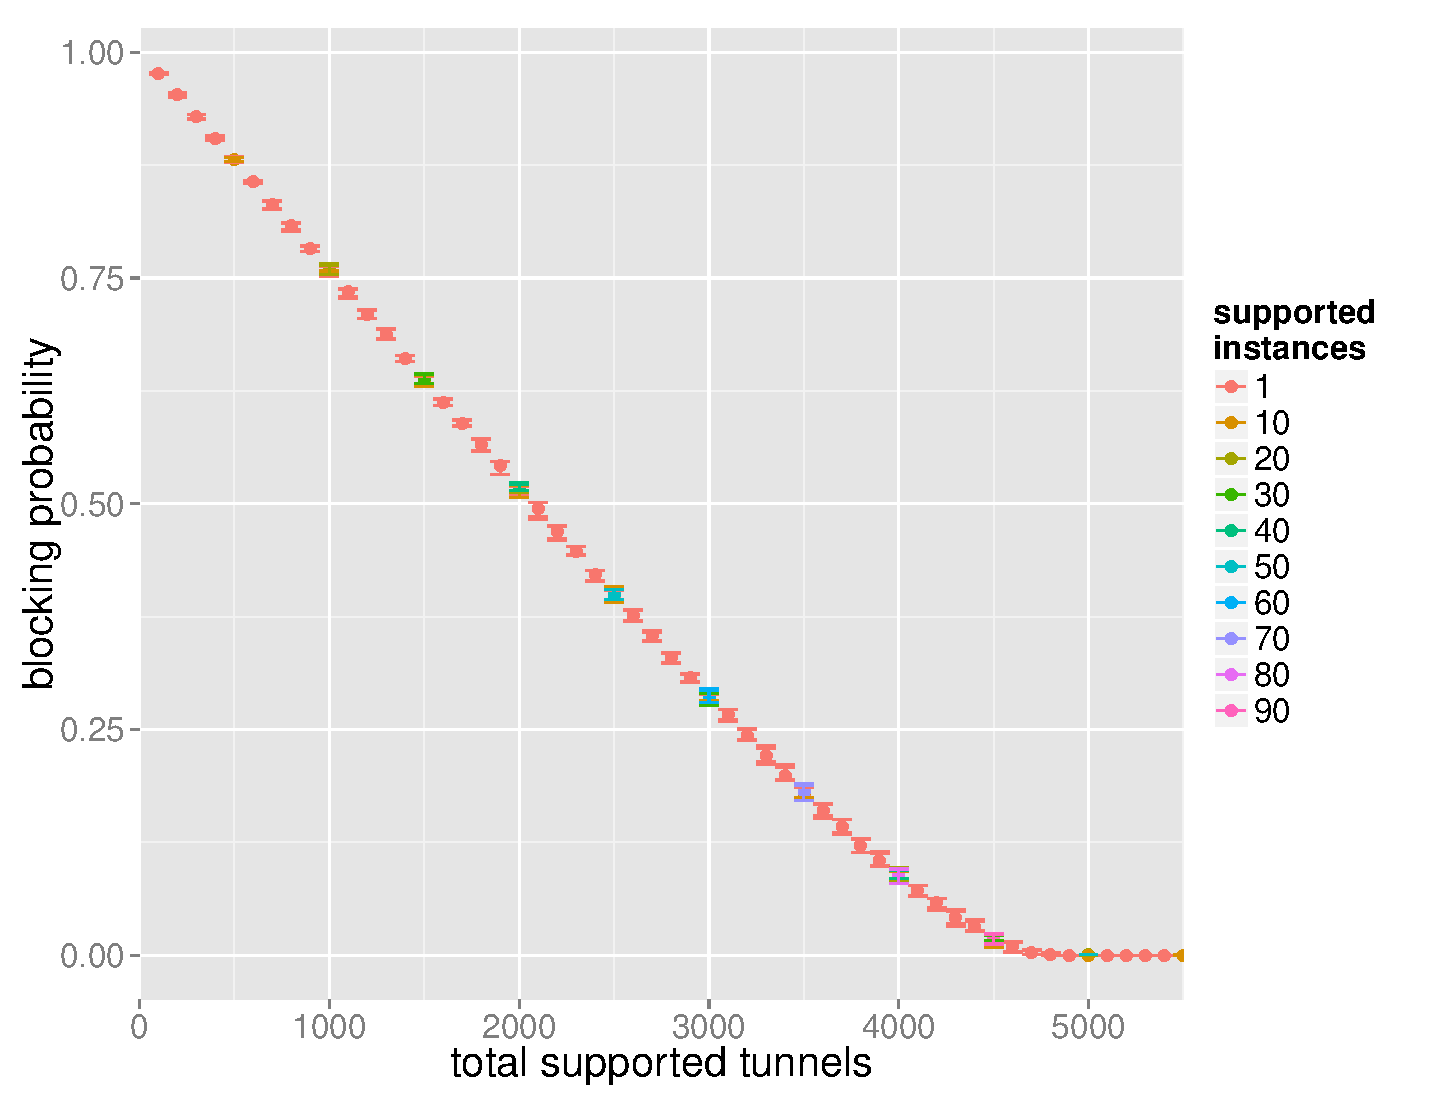
\includegraphics[width=1.0\textwidth]{images/feasiblemultiserver-blockprob.pdf}
  \caption{Comparison of the blocking probability of various server configurations.}
 \label{c4:fig:blockprob-multiserver}
\end{figure}

\begin{figure}[htb]
  \centering
  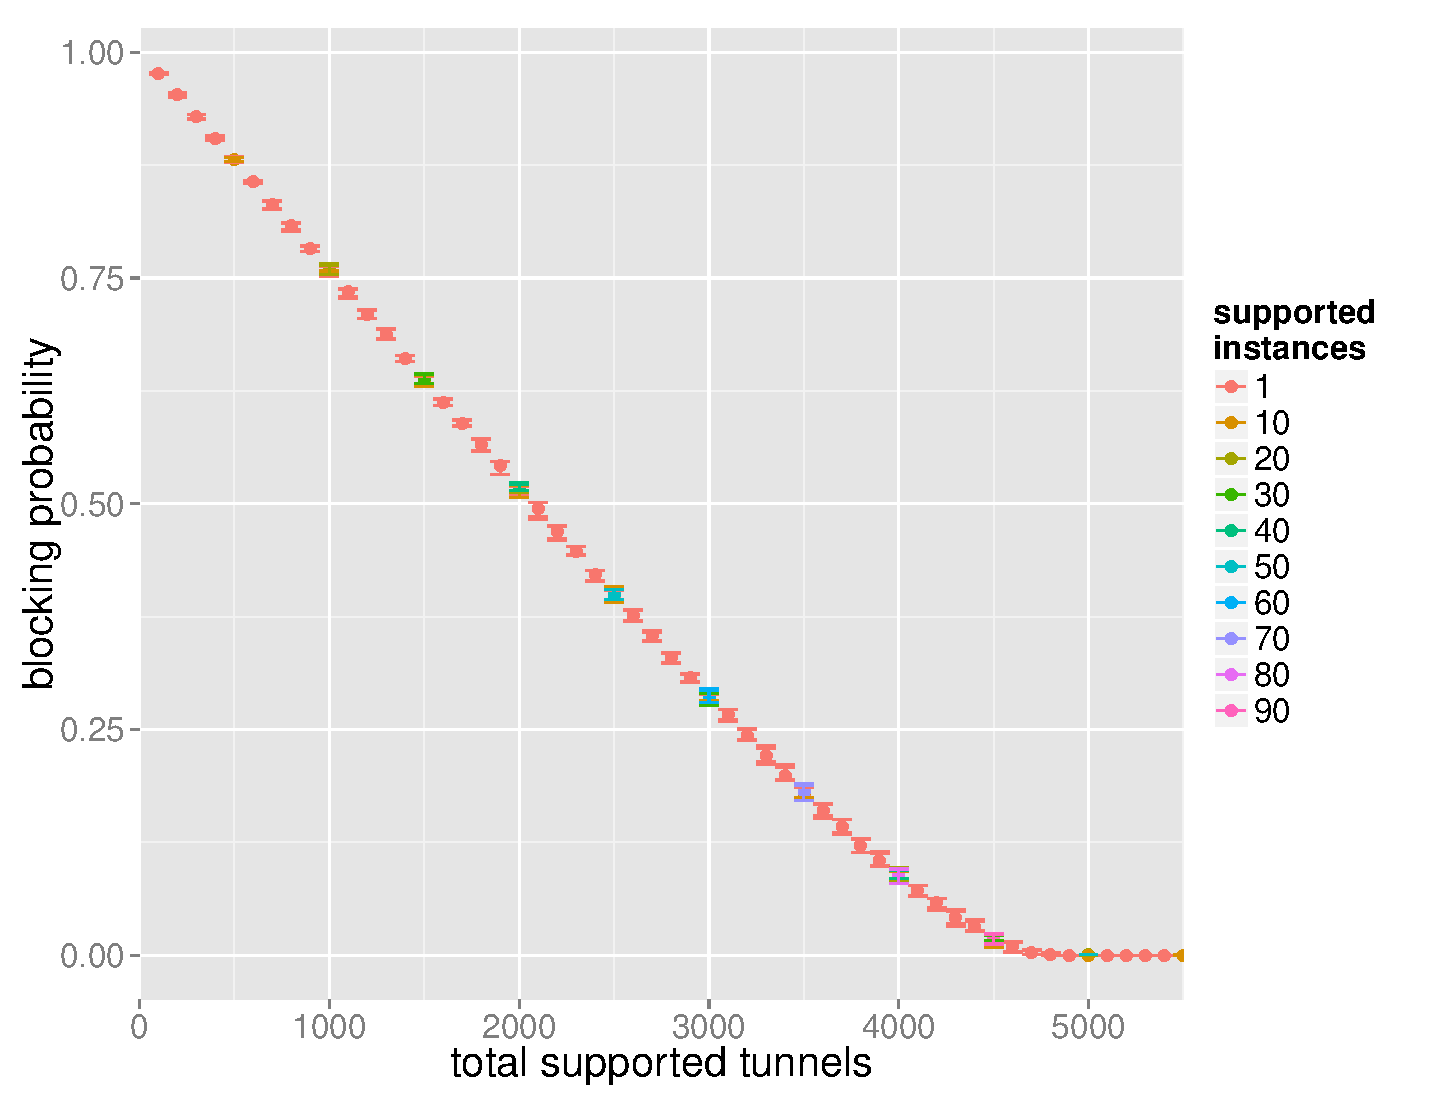
\includegraphics[width=1.0\textwidth]{images/feasiblemultiserver-blockprob.pdf}
  \caption{Comparison of the resource usage of various server configurations.}
 \label{c4:fig:res-usage-multiserver}
\end{figure}

\begin{figure}[htb]
  \centering
  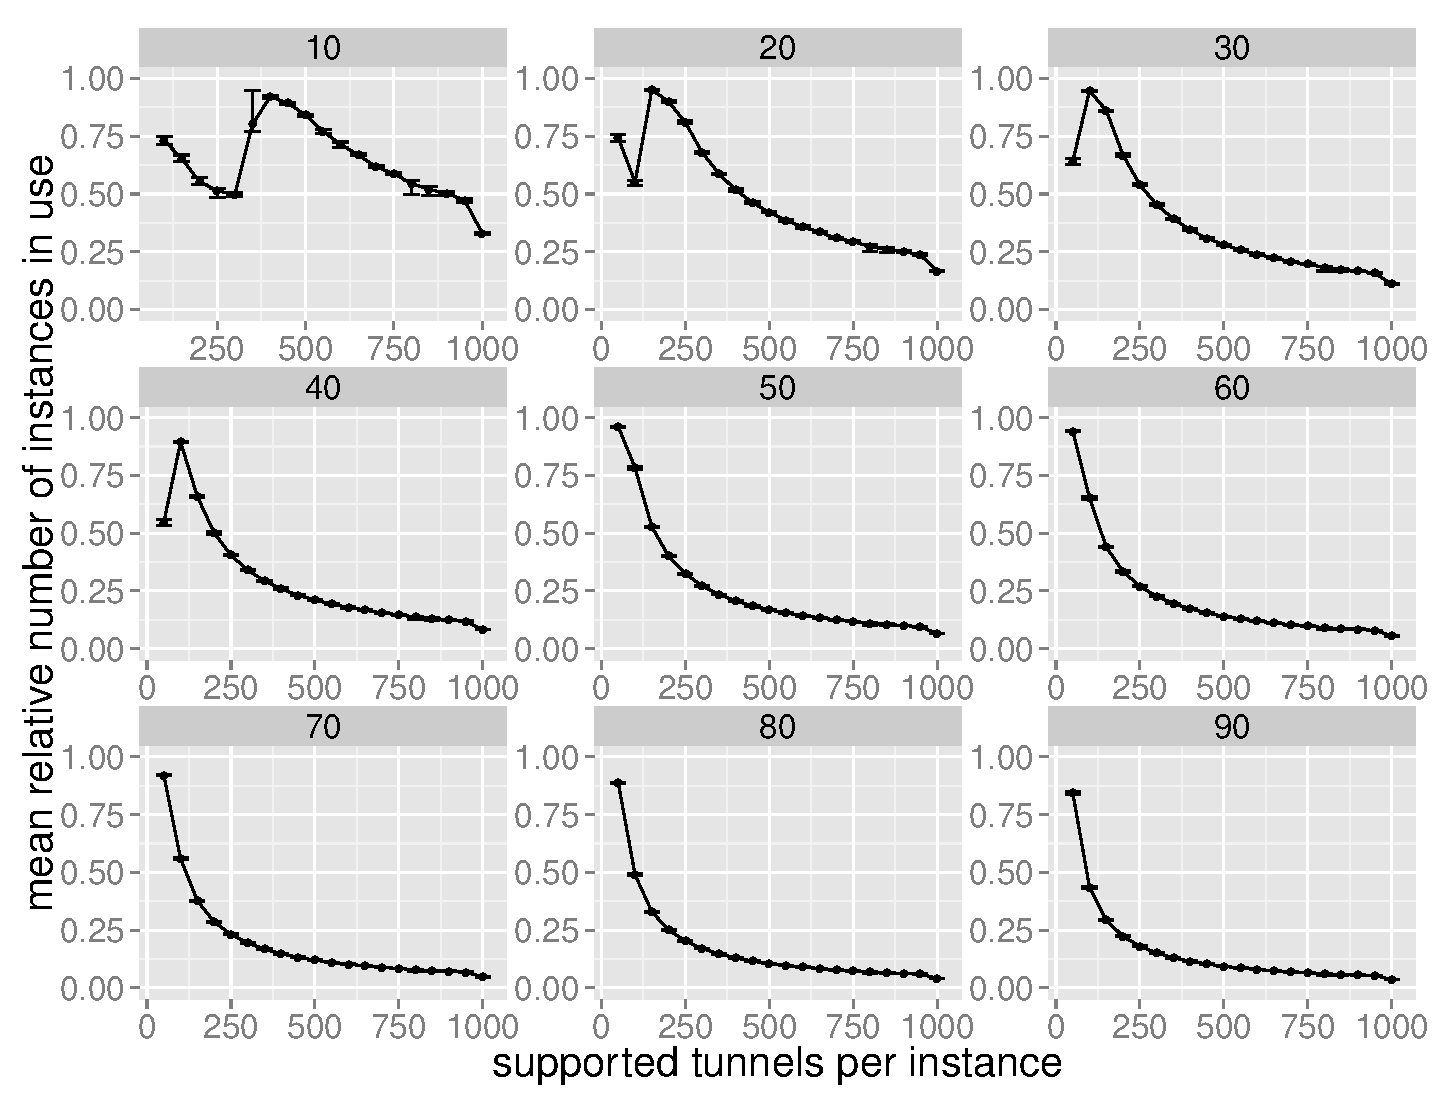
\includegraphics[width=1.0\textwidth]{images/instanceuse-mean.pdf}
  \caption{Mean instance usage of various server configurations.}
 \label{c4:fig:res-instance-usage-mean}
\end{figure}


